\chapter{Results and Discussions}
\section{User Interface Representation}
\begin{figure}[h]
	\centering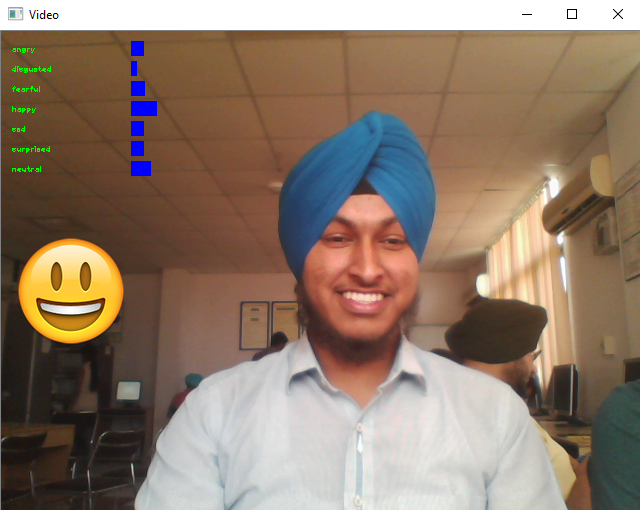
\includegraphics[scale=0.74]{images/ui.png}
	\caption{User Interface}
\end{figure}
Live emotion recognition through video is one of the most important key-points in human-machine interaction. To show the capabilities of the obtained network, an application is developed that can directly process web-cam footage through the final model.

With use of the aforementioned OpenCV face recognition program, the biggest appearing face from real-time video is tracked, extracted, and scaled to usable 48x48 input. This data is then fed to the input of the neural network model, which in its turn returns the values of the output layer. These values represent the likelihood that the each emotion is depicted by the user. The output with the highest value is assumed to be the current emotion of the user, and is depicted by an emotion on the left of the screen
\pagebreak

\subsection{Brief Description of Various Modules of the system}
\begin{figure}[h]
	\centering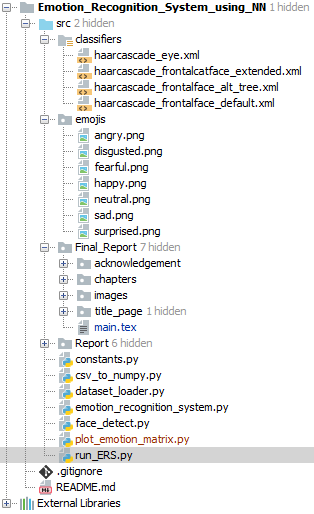
\includegraphics[scale=1]{images/file_tree.png}
	\caption{File Tree representing various System Modules}
\end{figure}

\textbf{face\_detect.py} - It is a script that runs on a input video stream may be on a video file or camera input , while using classifiers it detects the faces present in the video frame . The function in this file returns a NumPy array of detected faces per frame . These detected faces are then extracted out for further use.

\textbf{csv\_to\_numpy.py} - Since the data set provided to us is in CSV format , we need to convert that csv into numpy so that we can use it in our python module
The Dataset that we are using is radboud face dataset . This data set is the set of 64 Models having a set of 28,000 + pictures of people displaying 7 emotional expressions (angry, disgusted, fearful, happy, sad, surprised and neutral).

The dataset we are using consists of 2 types of data usages  - Training data and Test data. This script generates two models traing and test models . First one is used to train the machine and test data is used to verify the learning the machine.
\pagebreak

\textbf{emotion\_recognition\_system.py} - This is a script that contain all the model retailed settings. This file is the main file that user need to run to make the project working. It does two jobs:
\begin{enumerate}
	\item \textbf{Training}\\
	This part of the code is used to create and save the Deep Neural Network model from the dataset provided.
	\begin{figure}[h]
		\centering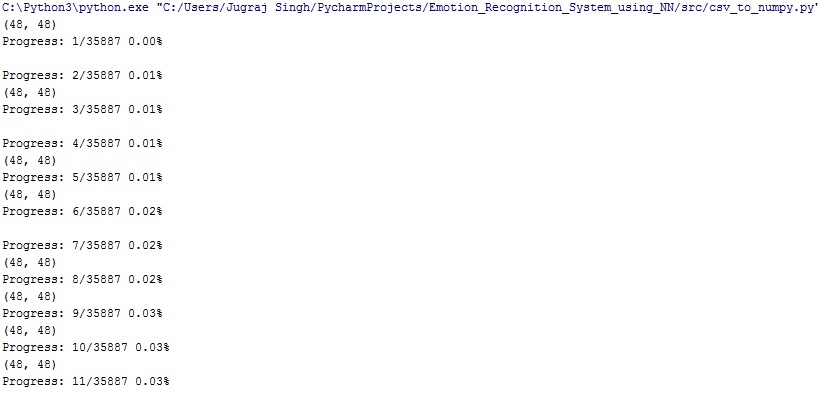
\includegraphics[scale=0.5]{images/csv_run.png}
		\caption{Running csv\_to\_numpy.py}
	\end{figure}\\This will create two train set and test set files used to train the model.
	\begin{figure}[h]
		\centering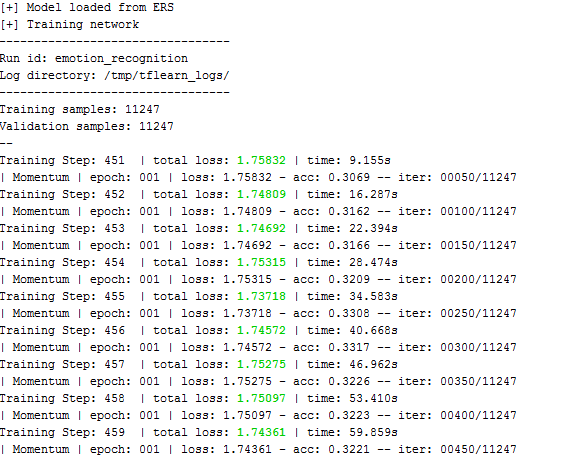
\includegraphics[scale=0.85]{images/ers_train.png}
		\caption{Running emotion\_recognition\_system.py train}
	\end{figure}
\pagebreak

	\item \textbf{Live Demo}
	\begin{figure}[h]
		\centering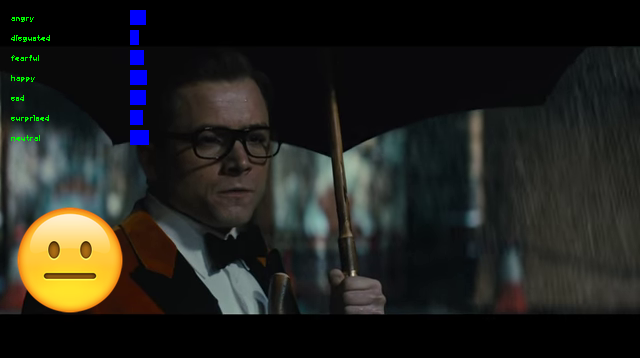
\includegraphics[scale=0.74]{images/angry_ui.png}
		\caption{User Interface Live Demo}
	\end{figure}
\end{enumerate} 

\textbf{dataset\_loader.py} - This is a script that contain all action needed to load the model into the system on running.

\textbf{haarcascade\_frontalface\_default.xml} - This is the classifer for the face detection model. It is a pre-trained classifer that eliminates the need to separately train a face detection classifier.